\section{Phase 4: PCA and Clustering}

\noindent \textbf{Timeline: December 4, 2025 -- January 2, 2026}

Following the causal audits of Phase 3, the project shifted from analyzing individual variables to discovering the \textbf{latent structures} that govern the Mexico City marketplace. This phase represents the critical convergence of the Agent's tacit domain knowledge and unsupervised machine learning, moving beyond standard administrative boundaries to identify organic "Neighborhoods of Profit." 

The mission of Phase 4 was twofold: first, to deconstruct the economic and topological archetypes of the market; and second, to execute a high-stakes forensic remediation of the coordinate data. This period was characterized by intense "Human-in-the-Loop" intervention, where automated discovery was audited against operational reality. The campaign culminated in a month-long data surgery—spanning the terminal days of 2025—to reconcile systemic semantic drift and geocoding entropy.

The structural investigation followed a five-stage progression:

\begin{itemize}[noitemsep, topsep=3pt]
    \item \textbf{Market Manifold Discovery:} Utilizing PCA to interrogate the high-dimensional feature space and identify the principal axes of market variance.
    \item \textbf{Economic Archetypes:} Deployment of K-Means to categorize the "DNA" of mission types based on yield and operational effort.
    \item \textbf{Topological Clustering:} Application of HDBSCAN to discover the organic density-based zones of the city.
    \item \textbf{Forensic Remediation:} A surgical strike to resolve the "Coordinate Crisis," correcting the systemic misalignment between address strings and geospatial points.
    \item \textbf{The Gold Palette Synthesis:} The formalization of the final geospatial intelligence layer, integrating machine-discovered clusters with human-curated strategic polygons.
\end{itemize}

-----
-----
PCA
-----
-----


\subsection{Feature Filtration: Redundancy and Signal Preparation}
To isolate pure signal, the 67-dimensional vector space was distilled to 54 variables through a three-stage filtration protocol:

\begin{enumerate}[noitemsep, topsep=3pt]
    \item \textbf{Variance Purge:} Quasi-constant features ($>99\%$ identical values), such as \texttt{is\_teens} and \texttt{is\_imputed}, were removed to eliminate computational dead weight.
    
    \item \textbf{Redundancy Resolution:} High-redundancy pairs ($r > 0.90$) were resolved through strategic selection. The project prioritized \textbf{Scale-Invariant Indexes} over raw currency and \textbf{Accumulated Earnings} over absolute clock time, identifying the former as a stronger behavioral driver. Geospatial coordinates were retained as indispensable geometric inputs.
    
    \item \textbf{Leakage Prevention:} Eight features with the \texttt{\_EDA} suffix were removed to prevent \textbf{Temporal Data Leakage} from post-facto mission outcomes.
\end{enumerate}

\noindent This 54-feature matrix serves as the foundation for Lasso-based selection and the subsequent principal component analysis. 

\subsection{Feature Selection: L1 Regularized Selection}
To identify the primary drivers of the agent's decision boundary, a \textbf{Lasso Regression (L1 Penalty)} was deployed across the 54-feature set. The selection identified \texttt{upfront\_fare}, \texttt{time\_to\_pickup\_sec}, and \texttt{home\_vector\_alignment\_score} as the dominant predictors.

A \textbf{Domain Override} was applied to align the machine with the operational reality of driving an Electric Vehicle. \textit{Distance} metrics were de-prioritized in favor of \textit{Time} metrics (e.g., \texttt{est\_trip\_time\_sec}), as time represents the definitive cost basis for the agent. 

Additionally, product category labels (\textit{Economy, Premium}) were intentionally excluded. This forces the model to identify the underlying economic and logistical causes of a decision rather than relying on categorical proxies. Features containing future outcome information were also purged to maintain a strictly predictive environment.

\subsubsection{Final Matrix and Normalization}
The dataset was distilled to a \textbf{19-feature whitelist}. Before Principal Component Analysis (PCA), variables such as fare, time, and density underwent \textbf{Log-Normal Transformations} to correct for distributional skewness, ensuring subsequent distance-based algorithms are not biased by outliers.

\begin{table}[H]
    \centering
    \scriptsize
    \begin{tabularx}{\textwidth}{X X X}
        \toprule
        \multicolumn{3}{c}{\textbf{The 19 Master Dimensions}} \\
        \midrule
        \texttt{consecutive\_rejects} & \texttt{eph\_complete\_index\_ML} & \texttt{log\_offer\_density\_10sec} \\
        \texttt{cycle\_avg\_dtp\_km} & \texttt{eph\_operational\_index} & \texttt{log\_time\_to\_pickup\_sec} \\
        \texttt{cycle\_cumulative\_net\_earnings} & \texttt{est\_trip\_time\_sec} & \texttt{log\_traffic\_index\_base\_120} \\
        \texttt{dispatch\_lead\_time\_sec} & \texttt{home\_vector\_alignment\_score} & \texttt{log\_upfront\_fare} \\
        \texttt{driver\_state\_at\_request\_fk} & \texttt{is\_long\_trip} & \texttt{session\_progress\_ratio} \\
        \texttt{time\_since\_last\_offer} & \texttt{is\_surge} & \texttt{total\_accumulated\_deadhead\_sec} \\
        \texttt{is\_turbo\_plus} & & \\
        \bottomrule
    \end{tabularx}
    \caption{Final high-signal feature set following L1 selection and expert-led pruning.}
    \label{tab:final_features}
\end{table}


\subsection{Market Manifold Analysis: Dimensionality Reduction via PCA}
Following feature curation, the 19-dimensional vector space was processed using \textbf{Principal Component Analysis (PCA)}. While subsequent clustering may utilize raw features for interpretability, PCA serves a critical methodological function: it ensures an \textbf{orthogonal} feature space where every dimension exerts an independent gravitational pull, removing the warping effect of correlated variables.

\subsubsection{Mathematical Foundation: The Spectral Theorem}
The PCA engine leverages the properties of the \textbf{Symmetric Covariance Matrix} ($C$). By applying the \textbf{Spectral Theorem}, the matrix is diagonalized ($C = Q \Lambda Q^T$), where $\Lambda$ is a diagonal matrix of \textbf{eigenvalues} and $Q$ is an orthogonal matrix of \textbf{eigenvectors}. This ensures that the resulting Principal Components are perfectly perpendicular (uncorrelated), and the market's total variance is cleanly sorted along the diagonal.

\subsubsection{Variance Allocation and Dimensional Cost}
Dimensionality reduction was modest, requiring 13 components to preserve 90\% of the variance from the original 19-feature set (Figure \ref{fig:scree_plot}). While standard PCA applications often exhibit heavy dominance in the first two components, the CDMX ecosystem reveals a \textbf{distributed eigenvalue structure}. The absence of a dominant principal component confirms the system's high dimensionality; the agent's decision logic is driven by the interplay of multiple orthogonal factors rather than a single primary variable.

\begin{figure}[H]
    \centering
    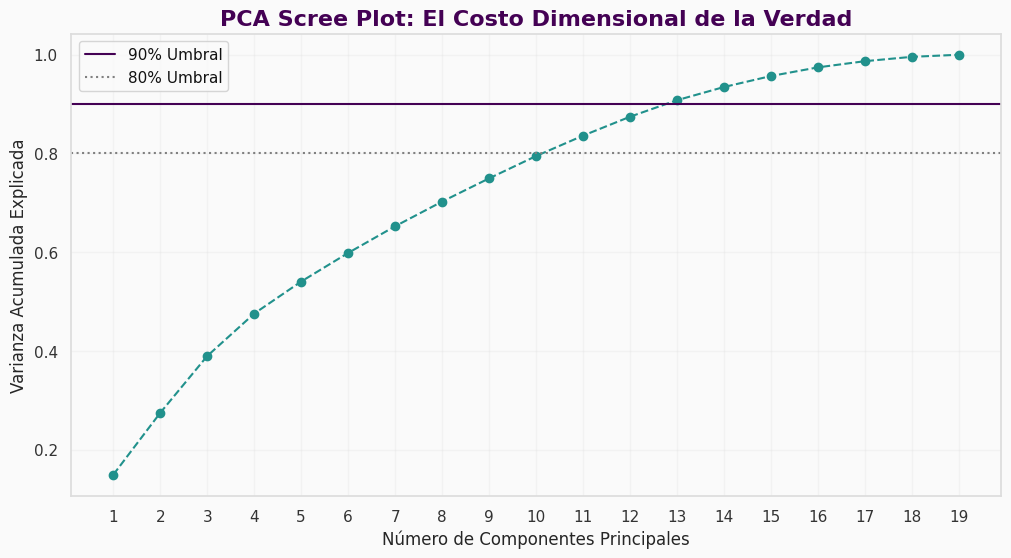
\includegraphics[width=0.7\textwidth]{pca_scree_plot.png}
    \caption{PCA Scree Plot. The gradual slope confirms a high-dimensional system where no single component explains more than 15\% of the total variance.}
    \label{fig:scree_plot}
\end{figure}


\subsubsection{Decoding the Market DNA (Principal Components)}
The first three components, explaining $\approx 40\%$ of the variance, define the universal mathematical structure of the total offer stream:

\begin{itemize}[noitemsep]
    \item \textbf{PC1: Time in Session:} Weighted by \texttt{session\_progress}, \texttt{deadhead}, and \texttt{cumulative\_earnings}. It separates early-session, low-friction states from high-search-accumulation segments toward the conclusion of a shift.
    \item \textbf{PC2: Volumetric Scale:} Weighted by \texttt{upfront\_fare} and \textit{estimated trip duration}. This axis distinguishes the physical magnitude of the mission, separating high-fare, long-duration missions from low-fare, high-turnover events.
    \item \textbf{PC3: Logistical Yield:} Weighted by \texttt{dispatch\_lead\_time} and the \textit{EPH Index}. It identifies opportunities where the financial compensation is high relative to the required operational time investment.
\end{itemize}

\begin{figure}[H]
     \centering
     \begin{subfigure}[b]{0.32\textwidth}
         \centering
         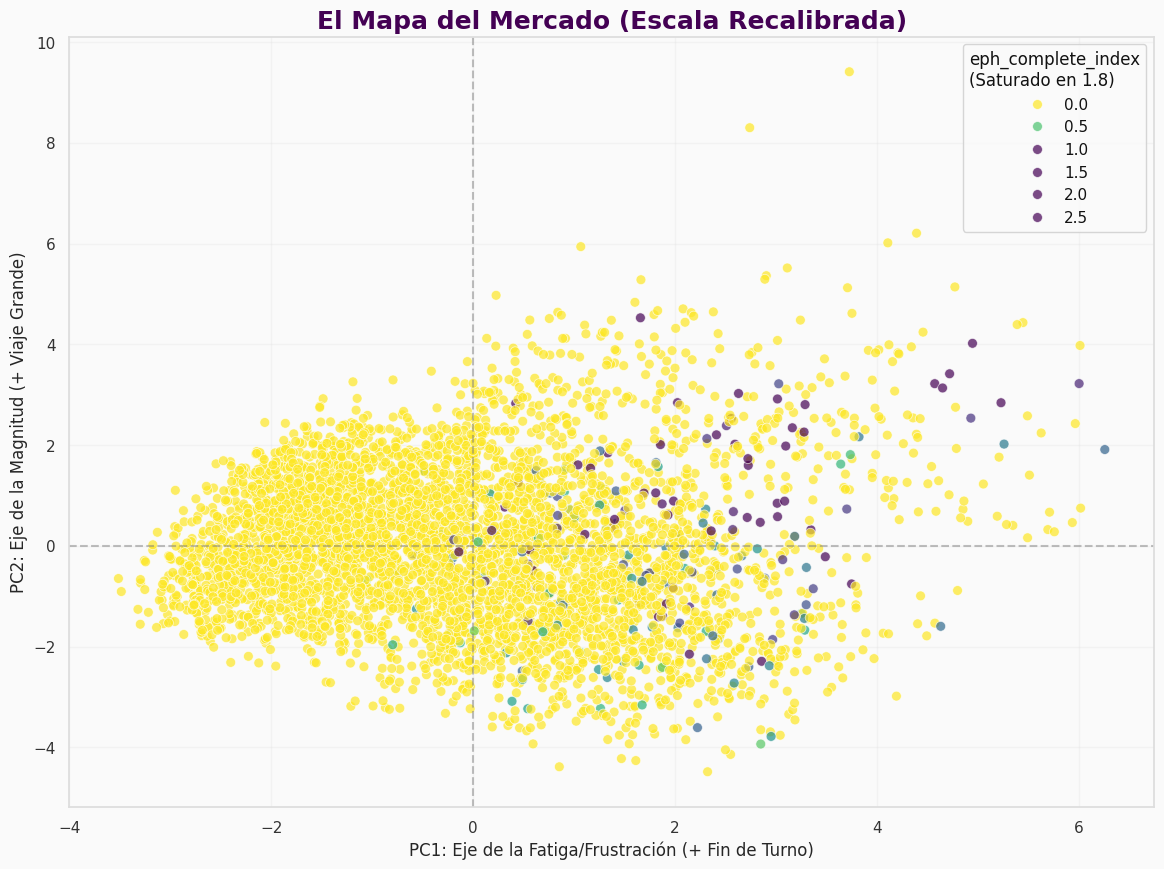
\includegraphics[width=\textwidth]{map_market.png}
         \caption{PC1 vs. PC2: Market Logic}
     \end{subfigure}
     \hfill
     \begin{subfigure}[b]{0.32\textwidth}
         \centering
         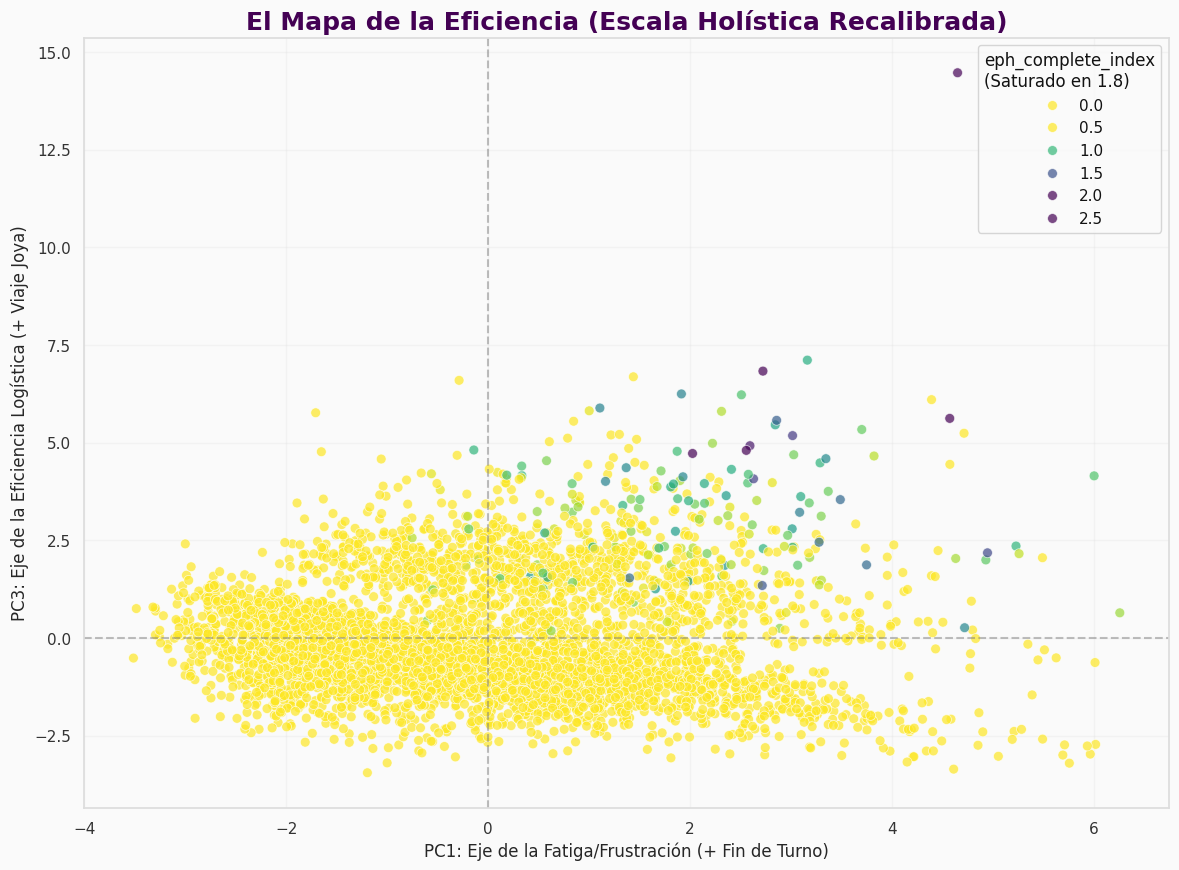
\includegraphics[width=\textwidth]{map_efficiency.png}
         \caption{PC1 vs. PC3: Efficiency Decay}
     \end{subfigure}
     \hfill
     \begin{subfigure}[b]{0.32\textwidth}
         \centering
         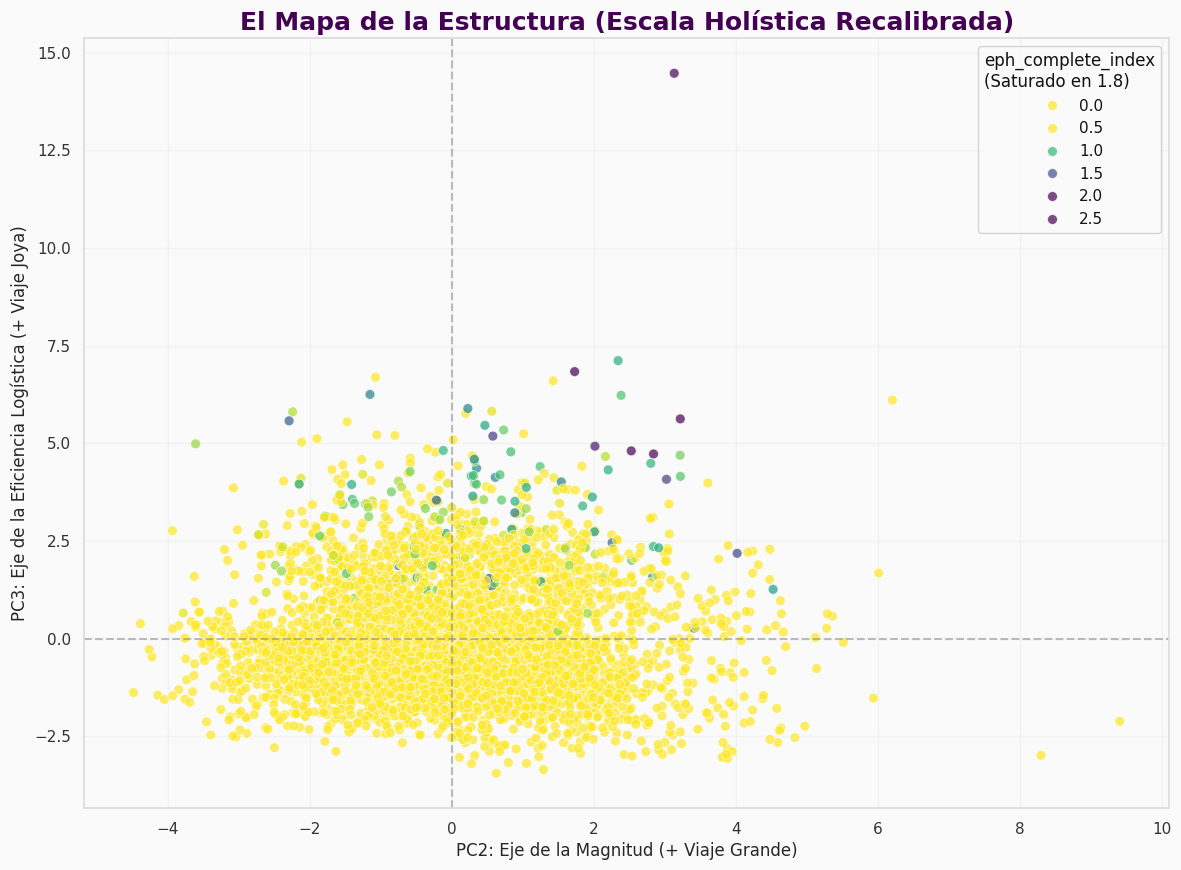
\includegraphics[width=\textwidth]{map_structure.png}
         \caption{PC2 vs. PC3: Yield Structure}
     \end{subfigure}
        \caption{Strategic Projection: Latent Market Manifolds. Color intensity represents the \texttt{eph\_complete\_index}. The maps deconstruct the interplay between session state, physical scale, and realized yield.}
        \label{fig:pca_maps}
\end{figure}

The projection of the feature space onto the primary principal components identifies the density regions where efficiency is maximized (Figure \ref{fig:pca_maps}):

\begin{enumerate}[noitemsep, topsep=3pt]
    \item \textbf{PC1 vs. PC2 (Market Logic):} Identifies how the available mission types shift as the agent accumulates operational time.
    \item \textbf{PC1 vs. PC3 (Efficiency Decay):} Indicates a correlation between fresh session states and peak efficiency.
    \item \textbf{PC2 vs. PC3 (Yield Structure):} Identifies that high-magnitude missions (High PC2) tend toward average yield, while high-efficiency outliers are primarily found in low-magnitude, high-turnover segments.
\end{enumerate}

\noindent This structural analysis confirms that peak performance is not uniformly distributed but occupies a specific coordinate space within the market manifold. These findings provide the objective boundaries for the \textbf{K-Means Strategic Archetypes} in the subsequent stage.


-
-
-
-
-END OF PCA -
-
-
-
-



-
-
-
-
- Start of K-Means -
-
-
-
-
-


\subsection*{K-Means Operational Clustering: Rejecting the Black Box}

An exploratory K-Means clustering algorithm was executed on the latent dimensions ($PC_1, PC_2, PC_3$). While the algorithm successfully partitioned the data across multiple tested $k$-universes ($k=2, 3, 4, 6$), the cluster profiles proved fundamentally uninterpretable for practical business strategy. Because each Principal Component is a linear combination of all 19 underlying features, the resulting clusters became opaque ``mixtures of mixtures.'' Ultimately, clustering on latent dimensions created a ``black box,'' making it impossible to reverse-engineer clear behavioral policies or business rules from abstract eigenvectors. \footnote{The evaluation of PCA-based clustering performance and the subsequent methodological pivot are documented in the Phase 4.1 notebook: \href{https://github.com/your-repo-placeholder}{[GitHub: Project Pienza - K-Means Trials]}.}

To resolve this interpretability barrier, a deliberate methodological pivot was executed to embrace a ``Crystal Box'' approach. PCA was formally abandoned as the input matrix for the clustering phase, with the methodology shifting to execute K-Means directly on the scaled raw features. 

An initial execution on the full 19-variable set identified a secondary interpretability barrier. While individual variables were transparent, defining mission archetypes based on 19 simultaneous dimensions resulted in a second "black box" outcome where high-level strategic signals were masked by marginal fluctuations in state and demand variables.

To resolve this, an \textbf{Incremental Clustering} strategy was adopted. The model was initially constrained to the "Naked Physics" of the transaction: \texttt{upfront\_fare}, \texttt{est\_trip\_time\_sec}, and \texttt{est\_trip\_dist\_km}, excluding all algorithmic incentives or agent-state features. Applying the principle of \textbf{Occam's Razor}, the project identified that the market's fundamental structure is almost entirely dictated by these spatio-temporal magnitudes.

A comparative analysis between the \textbf{Elbow Method} and \textbf{Silhouette Score} was conducted to determine the optimal cluster count ($k$) for the CDMX marketplace (Figure \ref{fig:k_selection}).

\begin{figure}[H]
    \centering
    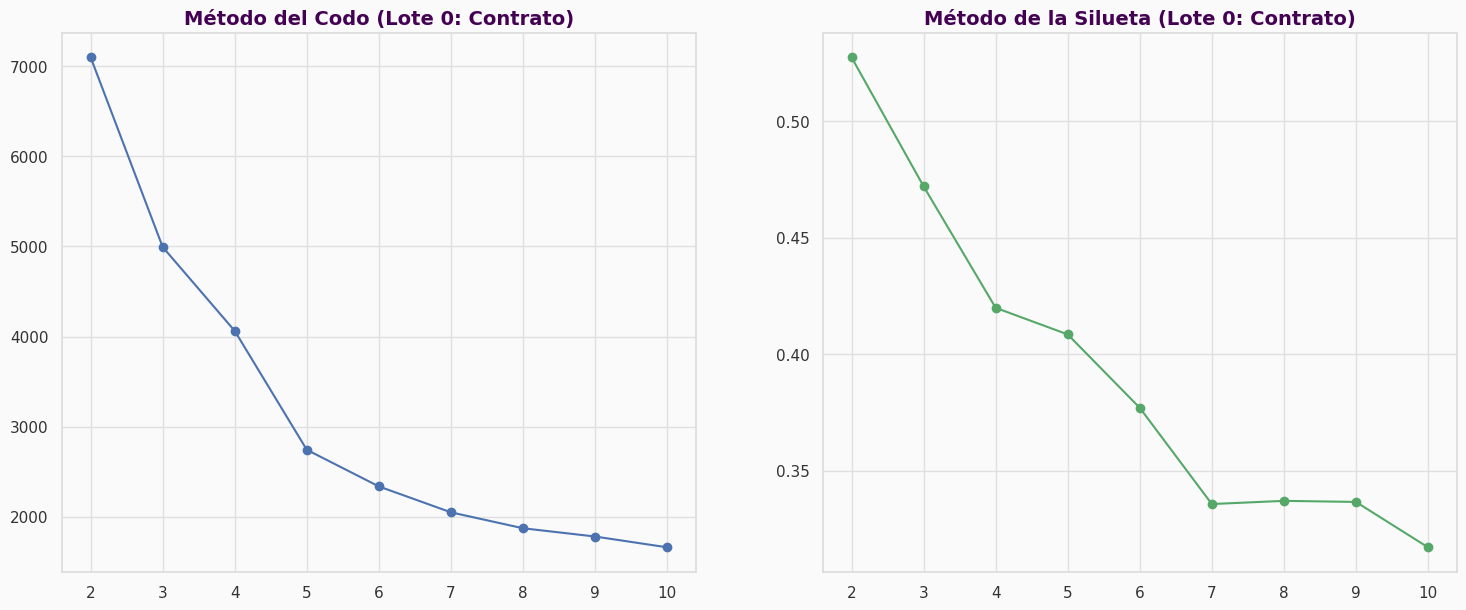
\includegraphics[width=\textwidth]{fig_k_selection.png} 
    \caption{Hyperparameter Tournament ($k$): Elbow Method and Silhouette Score analysis for the "Naked Physics" feature set.}
    \label{fig:k_selection}
\end{figure}

\begin{itemize}
    \item \textbf{Mathematical Baseline ($k=2$):} The Silhouette Score indicated a peak at $k=2$. While geometrically optimal, this trivial binary split (Short vs. Long missions) was rejected for its failure to capture the nuanced operational regimes that dictate profitability.
    \item \textbf{Expert-Led Resolution ($k=6$):} A visual inspection of the Elbow Plot identified a significant reduction in inertia occurring at $k=6$. This higher-resolution setting was ratified as the optimal choice, as it provided sufficient granularity to decode the transition between distinct states in the agent’s policy.
\end{itemize}

The analysis revealed that the marketplace fractures into six distinct physical tiers based on temporal magnitude and logistical scale (Table \ref{tab:mission_tiers}). 

\begin{table}[H]
    \centering
    \small
    \begin{tabular}{l l}
        \toprule
        \textbf{Designation} & \textbf{Median Duration}\footnotemark \\
        \midrule
        \texttt{Tier 1} & 12 minutes \\
        \texttt{Tier 2} & 25 minutes \\
        \texttt{Tier 3} & 40 minutes \\
        \texttt{Tier 4} & 56 minutes \\
        \texttt{Tier 5} & 80 minutes \\
        \texttt{Tier 6} & 224+ minutes \\
        \bottomrule
    \end{tabular}
    \caption{CDMX market archetypes based on $K=6$ clustering.} 
    \label{tab:mission_tiers} 
\end{table}
\footnotetext{Median duration is derived from multi-dimensional $K$-Means centroids rather than deterministic binning. Consequently, observations with identical durations may be assigned to different tiers based on the specific variance in fare magnitude and trip distance.}

Cross-referencing the Agent's historical rejections against these six tiers provides empirical evidence of a \textbf{non-stationary decision policy}. The primary decision driver shifts dynamically as the physical scale of the offer increases:

\begin{itemize}[noitemsep, topsep=3pt]
    \item \textbf{Low-Magnitude Missions (Tiers 1--3):} Rejections are primarily governed by the \textbf{Economic Layer}. For "Sprints" (Tier 1), the dominant friction point is \texttt{low\_profitability} ($\approx 44\%$ of rejections). The Agent's priority is yield-per-minute efficiency. \footnote{Although Tier 1 missions exhibit the highest quoted EPH, the agent utilized historical operational knowledge identifying these as low-yield events once uncompensated search and pickup overheads are factored in.}
    \item \textbf{High-Magnitude Missions (Tiers 4--6):} Rejections are governed strictly by the \textbf{Geospatial Layer}. As trip duration approaches the one-hour threshold, economic metrics are ignored. For Tier 5 missions, \texttt{dropoff\_non\_operational} accounts for $>98\%$ of rejections, reflecting a pure destination-based strategy.
\end{itemize}

A review of the base fare structure across these tiers reveals two distinct algorithmic laws governing the market (Figure \ref{fig:pricing_physics}). \footnote{Base fare is isolated by removing all incentives from the upfront quote to ensure a normalized comparison of structural pricing.}

\begin{figure}[H]
    \centering
    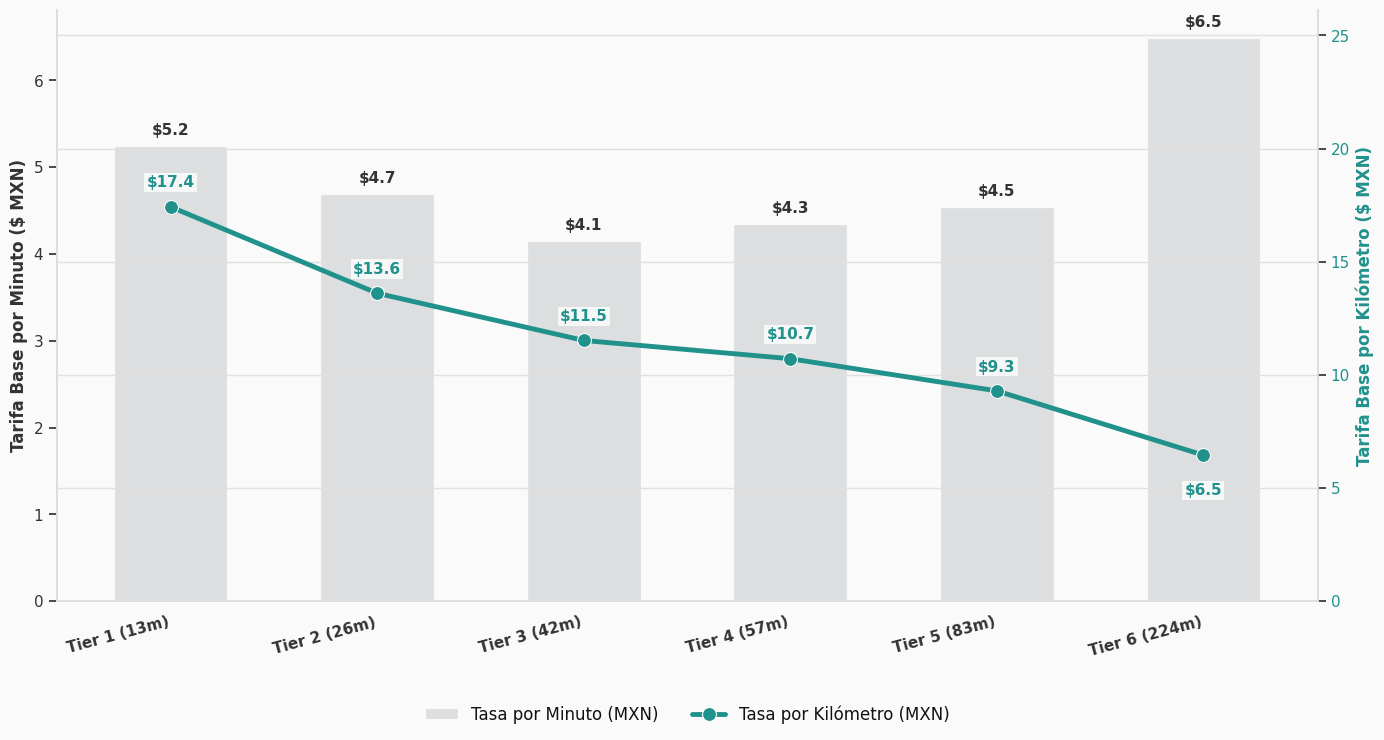
\includegraphics[width=\textwidth]{fig_pricing_physics.png} 
    \caption{The Physics of Pricing: Mean yield per minute and kilometer across mission tiers. The dual-axis plot illustrates the systematic decay of distance-based rewards and the U-curve of temporal compensation.}
    \label{fig:pricing_physics}
\end{figure}

\begin{enumerate}[noitemsep]
    \item \textbf{Compensation per kilometer:} exhibits an inverse relationship with mission scale. Yield begins at \textbf{\$17.4 MXN/km} for Tier 1 and collapses to \textbf{\$6.5 MXN/km} for Tier 6. 
    \item \textbf{Compensation per minute:} follows a non-linear "U" structure. Rates are high for Sprints (\textbf{\$5.2 MXN/min}) to offset fixed search costs, reach a minimum for mid-range urban missions (\$4.1/min), and increase again for Tier 5 and Tier 6.
\end{enumerate}


\subsubsection{Yield Analysis Across Operational Tiers}
To evaluate the economic viability of the discovered archetypes, the analysis measured the performance of each tier against the \textbf{\$200/hr North Star} benchmark. As shown in Figure \ref{fig:yield_tiers}, the transition from quoted potential to holistic outcome identifies how trip duration dictates final efficiency.

\begin{figure}[H]
    \centering
    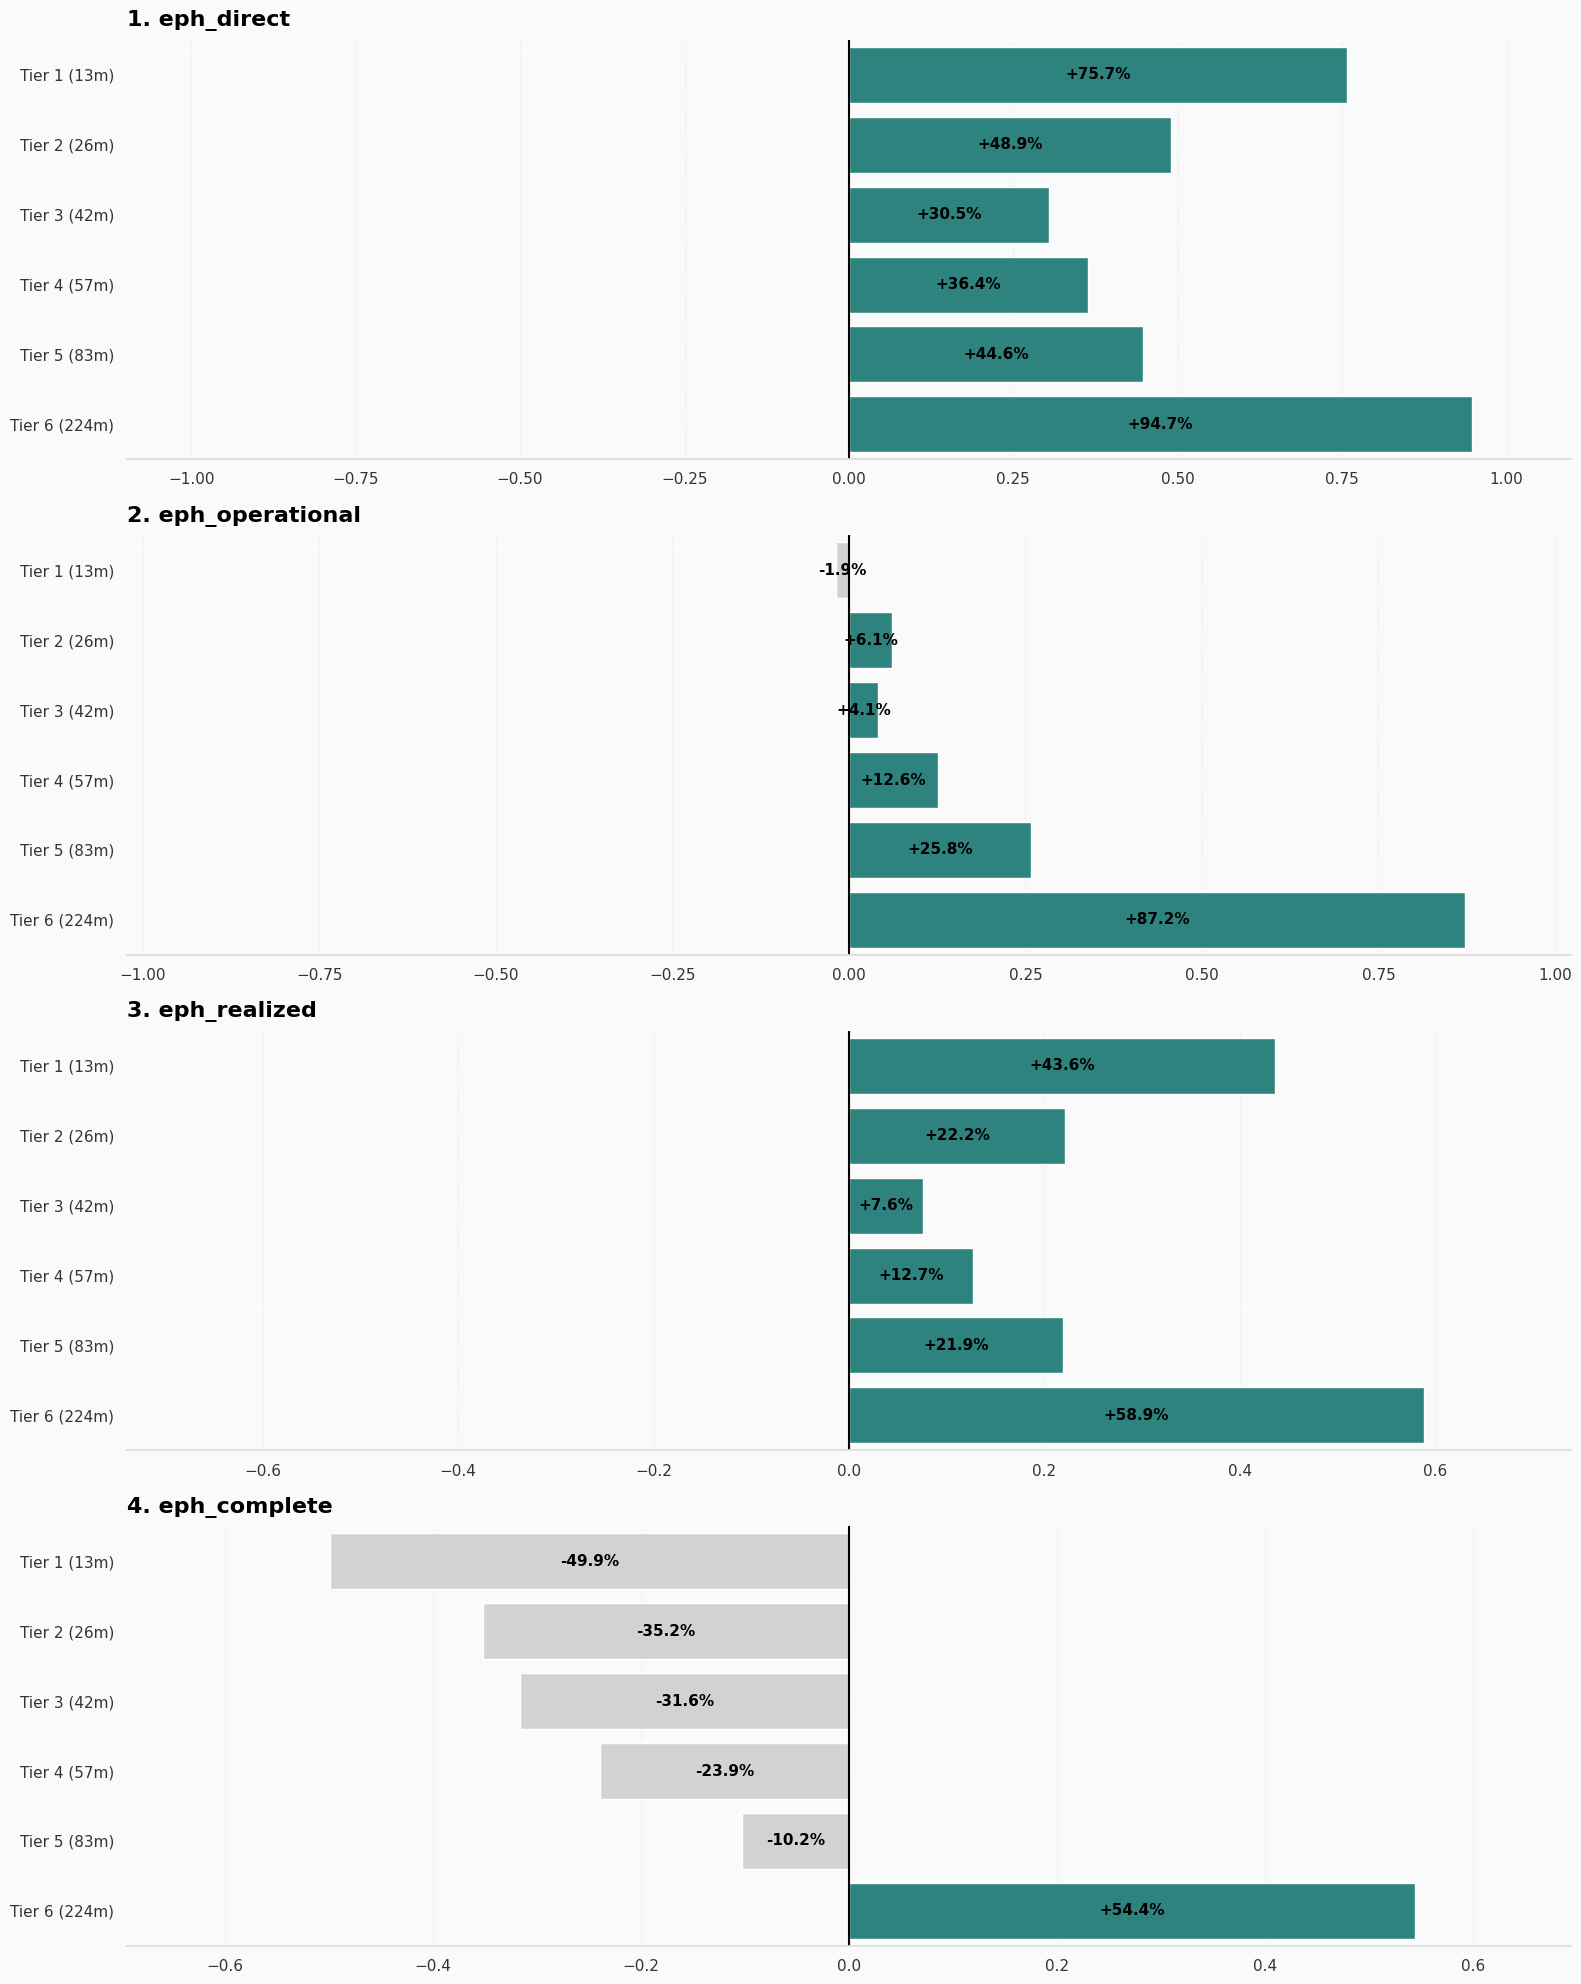
\includegraphics[width=0.85\textwidth]{fig_yield_tiers.png} 
    \caption{Yield Variance by Mission Tier. Bars represent the percentage deviation relative to the \$200/hr target. Negative values indicate a yield below the North Star threshold rather than a net financial loss.}
    \label{fig:yield_tiers}
\end{figure}

The result identifies the \textbf{Amortization of Deadhead} as the primary driver of mission efficiency:
\begin{itemize}[noitemsep, topsep=3pt]
    \item \textbf{Search-Intensive Sprints (Tier 1):} Although quoted at $+75.7\%$ above the target, the realized yield collapses to $-49.9\%$. In these short-duration missions, the uncompensated temporal investment (searching and pickup) outweighs the revenue-generating phase.
    \item \textbf{Scale Resilience (Tiers 4-6):} Long-duration missions demonstrate the highest capacity to meet the sustainability benchmark, successfully diluting fixed search costs across a larger revenue base. However, the yield for Tier 6 represents rare interstate statistical anomalies. This specific metric excludes the massive time required to return back the city, which would halve the realized yield in a full-cycle context.
\end{itemize}


 \noindent Having established the fundamental economic archetypes, the study proceeds to the discovery of the geospatial dimension to identify the organic operational zones of the city.

\vspace{0.4cm}
\rule{\linewidth}{0.4pt}



-
-
-
-
- END of K-Means -
-
-
-
-
-

--

-
-
-
-
HDBSCAN
----
-
-
-
-
-
-


\subsection{Unsupervised Topology: Organic Zone Discovery}
The geospatial objective was to transform $\approx 4,700$ dropoff coordinates into a \textbf{Topological Operational Model}. This strategic mapping converts raw spatial distributions into a high-value categorical feature (\texttt{zone\_id}) to enable the predictive pipeline to recognize geographic intent.

While \textbf{DBSCAN} was chosen initially, it resulted in data fragmentation that made no business logic. Therefore, the architecture was upgraded to \textbf{HDBSCAN} (Hierarchical DBSCAN), which dynamically extracts clusters across multiple density scales. HDBSCAN naturally capturared Mexico's City complex operational reality by identifying 45 granular high-resolution micro-clusters. 


In an attempt to achieve 100\% feature coverage a \textbf{K-Nearest Neighbors (KNN)} classifier was deployed to re-assign unclustered points to their nearest cluster. This algorithmic fallback was identified as a functional failure. By forcing these points into the nearest core based strictly on Euclidean distance, the resulting topology lost all operational relevance. 

While the HDBSCAN model was mathematically sound and aligned with the operational reality, a deep validation audit was conducted to verify semantic alignment. The coordinate-based clusters were cross-referenced against the raw \texttt{dropoff\_address} text strings. This audit identified a systemic data integrity failure. Inspection of the \textit{AICM} (Airport) cluster revealed addresses belonging to distant parts of the city, such as Cuajimalpa. While the algorithm had correctly identified density clusters, the underlying geocoded coordinates had become decoupled from their true textual addresses during the upstream ingestion phase. This "Garbage In, Garbage Out" (GIGO) corruption invalidated the unsupervised topology and necessitated a major remediation campaign.

To restore geospatial integrity, a Human-in-the-Loop (HITL) approach was adopted. The Agent manually architected 73 custom heuristic polygons to serve as the ultimate spatial ground truth. This manual intervention solved both pipeline crises simultaneously. First, it guaranteed that every coordinate within the operational radius would be deterministically mapped to a valid zoneid, effectively eliminating the orphaned data problem. Second, it provided a rigid spatial framework that drastically accelerated the data auditing process. By cross-referencing the raw dropoffaddress strings contained within each newly drawn HITL polygon, anomalous and corrupted coordinates were instantly isolated and rectified. Consequently, this initiated a deep remediation campaign to reconcile and purify the entire geospatial dataset.


\subsection{Geospatial Remediation: Root Cause Analysis}
Validation of the initial clustering results identified a systemic integrity failure. This discovery triggered a deep \textbf{Root Cause Analysis (RCA)} that identified three compounding failure vectors:

\begin{enumerate}[noitemsep, topsep=3pt]
    \item \textbf{Validation Gap:} The initial Phase 1 acquisition utilized forward geocoding without a reverse-validation step, allowing API hallucinations to persist in the dataset.
    \item \textbf{Semantic Entropy:} Contradictory neighborhood labels in the platform's raw address strings (e.g., \textit{``Calle Insurgentes Tacubaya, Condesa/Roma''}) caused the black-box API to default coordinates to incorrect municipalities.
    \item \textbf{Propagation Error:} A logical bug during the Phase 2B jittering stage caused hundreds of distinct textual addresses to collapse into a single, identical coordinate point.
\end{enumerate}

\subsubsection{Diagnostic Engineering}
To isolate the corrupted records, a diagnostic SQL query was engineered based on a strict relational rule: \textbf{Fixed Coordinates + Changing Text = Error}. By grouping identical coordinates and counting distinct address strings, the project isolated the specific records requiring intervention without compromising the healthy data.

\begin{lstlisting}[language=SQL, caption={Diagnostic Query: Isolating Jitter Propagation Errors}]
-- Logic: If one exact coordinate belongs to multiple distinct text addresses, it is corrupted.
SELECT offer_id,
    CASE WHEN c.num_pickups > 1 THEN 'PICKUP_ERROR'
         WHEN c.num_dropoffs > 1 THEN 'DROPOFF_ERROR'
    END as diagnostic_flag
FROM offers o
JOIN (
    SELECT pickup_lat, pickup_lon, dropoff_lat, dropoff_lon,
        COUNT(DISTINCT pickup_address) as num_pickups,
        COUNT(DISTINCT dropoff_address) as num_dropoffs
    FROM offers
    GROUP BY pickup_lat, pickup_lon, dropoff_lat, dropoff_lon
    HAVING COUNT(DISTINCT pickup_address) > 1 OR COUNT(DISTINCT dropoff_address) > 1
) c ON o.pickup_lat = c.pickup_lat AND o.dropoff_lat = c.dropoff_lat;
\end{lstlisting}

\subsubsection{Remediation Architecture: The Delta Check Pipeline}
To rescue the dataset, a two-stage \textbf{Human-in-the-Loop (HITL)} reconciliation pipeline was executed across all 9,530 coordinate pairs:

\begin{enumerate}[noitemsep]
    \item \textbf{Geospatial Delta Check:} A secondary baseline was established by re-geocoding the dataset in a dedicated cloud environment. A \textbf{Delta Check} was implemented to calculate the distance (in meters) between original and new coordinates. Only records exceeding a severe geographic threshold were flagged for manual review.
    \item \textbf{Deterministic Overwrite:} A bespoke ETL tool managed the manual corrections. The system staged flagged conflicts alongside verified context, enabling the agent to surgically overwrite corrupted coordinate pairs in the source tables while preventing manual entry errors.
\end{enumerate}

\noindent \textit{Outcome: This intervention successfully corrected over 1,500 corrupted rows—nearly one-third of the operational history. The canonical Source of Truth was updated with this purified dataset, allowing the clustering pipeline to be re-executed with high-fidelity results.}

\vspace{0.4cm}
\rule{\linewidth}{0.4pt}


\subsection{Gold Palette Synthesis}
Following coordinate remediation, the project finalized the \textbf{Gold Palette}—the highest tier of geospatial intelligence. This layer provides the supervised models with a dual-perspective of the city, combining machine-learned density with human-curated strategic boundaries.

\subsubsection{Topological vs. Strategic Mapping}
The resulting geospatial features serve distinct roles within the predictive pipeline:

\begin{enumerate}[noitemsep, topsep=3pt]
    \item \textbf{Structural Discovery (\texttt{hdbscan\_id}):} As illustrated in Figure \ref{fig:geospatial_intelligence}(a), the HDBSCAN algorithm identified 45 organic operational hubs. These micro-zones represent an unbiased discovery of where market activity actually concentrates.
    \item \textbf{Strategic Guardrails (\texttt{polygon\_id}):} As shown in Figure \ref{fig:geospatial_intelligence}(b), these clusters were formalized into 73 hand-crafted polygons. By enforcing crisp geometric boundaries, these polygons act as a countermeasure against overfitting, requiring the model to learn the economic attributes of a neighborhood rather than memorizing coordinate noise.
\end{enumerate}

\begin{figure}[H]
     \centering
     \begin{subfigure}[b]{0.48\textwidth}
         \centering
         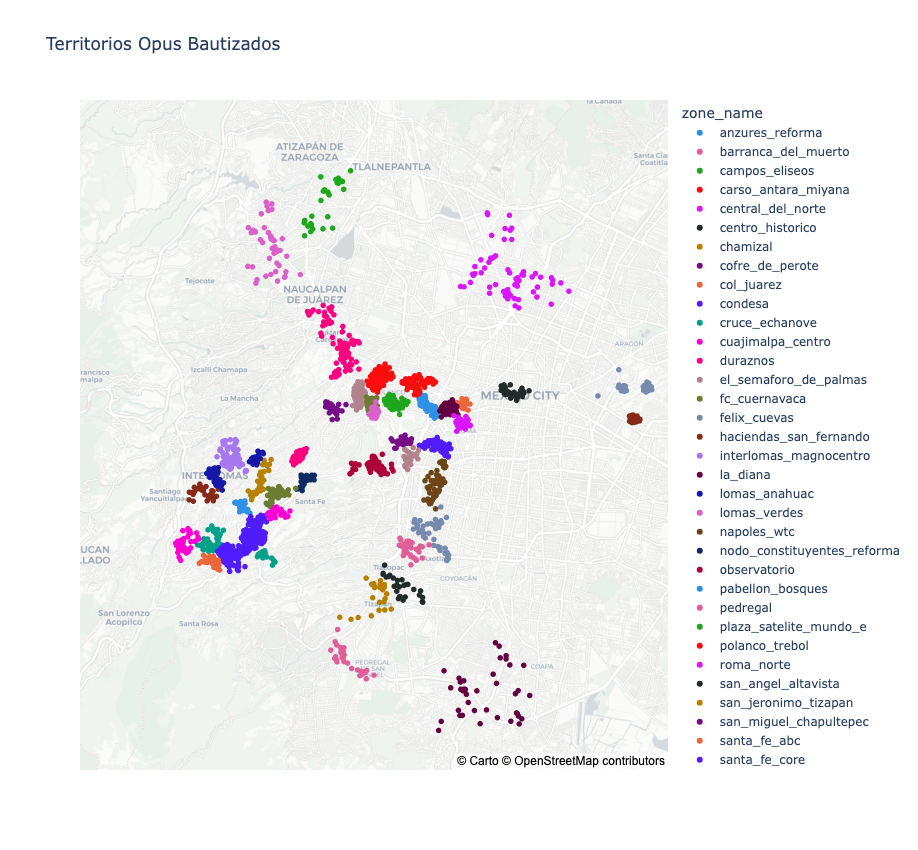
\includegraphics[width=\textwidth]{fig_hdbscan.png}
         \caption{HDBSCAN clusters assigned operational names.}
     \end{subfigure}
     \hfill
     \begin{subfigure}[b]{0.48\textwidth}
         \centering
         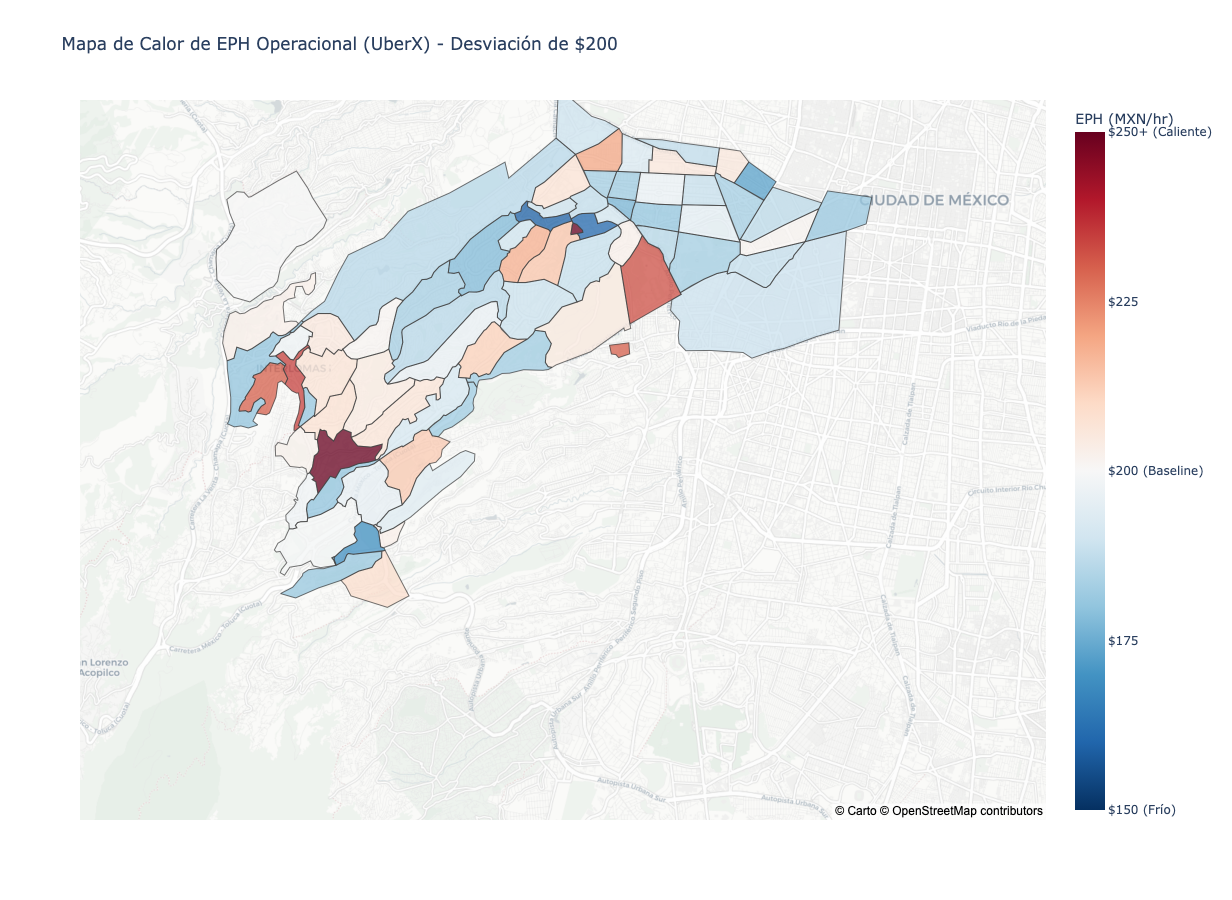
\includegraphics[width=\textwidth]{fig_polygons.png}
         \caption{Realized yield variance by polygon (\$200/hr baseline).}
     \end{subfigure}
     \caption{Geospatial Intelligence Layer. The synthesis of machine-learned clusters and human-curated strategic polygons defines the ``Gold Palette.''}
     \label{fig:geospatial_intelligence}
\end{figure}

\subsubsection{Economic Geography Findings}
The realized yield heatmap identifies specific regions of high profitability. Clusters within \textit{Interlomas}, the \textit{Santa Fe Core}, and the \textit{Polanco-Lomas} axis exhibit consistent performance exceeding the \$200/hr benchmark, while peripheral and unassigned zones identify areas of systemic yield erosion. 

\noindent \textit{Outcome: The integration of \texttt{hdbscan\_id} and \texttt{polygon\_id} provides the high-purity geospatial signal required for the supervised modeling campaign in Phase 5.}

\vspace{0.4cm}
\rule{\linewidth}{0.4pt}